% Created 2021-09-12 Sun 22:49
% Intended LaTeX compiler: xelatex
\documentclass[letterpaper]{article}
\usepackage{graphicx}
\usepackage{grffile}
\usepackage{longtable}
\usepackage{wrapfig}
\usepackage{rotating}
\usepackage[normalem]{ulem}
\usepackage{amsmath}
\usepackage{textcomp}
\usepackage{amssymb}
\usepackage{capt-of}
\usepackage{hyperref}
\usepackage[margin=1in]{geometry}
\usepackage{fontspec}
\usepackage{indentfirst}
\setmainfont[ItalicFont = LiberationSans-Italic, BoldFont = LiberationSans-Bold, BoldItalicFont = LiberationSans-BoldItalic]{LiberationSans}
\newfontfamily\NHLight[ItalicFont = LiberationSansNarrow-Italic, BoldFont       = LiberationSansNarrow-Bold, BoldItalicFont = LiberationSansNarrow-BoldItalic]{LiberationSansNarrow}
\newcommand\textrmlf[1]{{\NHLight#1}}
\newcommand\textitlf[1]{{\NHLight\itshape#1}}
\let\textbflf\textrm
\newcommand\textulf[1]{{\NHLight\bfseries#1}}
\newcommand\textuitlf[1]{{\NHLight\bfseries\itshape#1}}
\usepackage{fancyhdr}
\pagestyle{fancy}
\usepackage{titlesec}
\usepackage{titling}
\makeatletter
\lhead{\textbf{\@title}}
\makeatother
\rhead{\textrmlf{Compiled} \today}
\lfoot{\theauthor\ \textbullet \ \textbf{2021-2022}}
\cfoot{}
\rfoot{\textrmlf{Page} \thepage}
\titleformat{\section} {\Large} {\textrmlf{\thesection} {|}} {0.3em} {\textbf}
\titleformat{\subsection} {\large} {\textrmlf{\thesubsection} {|}} {0.2em} {\textbf}
\titleformat{\subsubsection} {\large} {\textrmlf{\thesubsubsection} {|}} {0.1em} {\textbf}
\setlength{\parskip}{0.45em}
\renewcommand\maketitle{}
\author{Houjun Liu}
\date{\today}
\title{Van De Graff Generators}
\hypersetup{
 pdfauthor={Houjun Liu},
 pdftitle={Van De Graff Generators},
 pdfkeywords={},
 pdfsubject={},
 pdfcreator={Emacs 28.0.50 (Org mode 9.4.4)}, 
 pdflang={English}}
\begin{document}

\maketitle


\section{A Van De Graff Generator}
\label{sec:org357a17c}
\begin{figure}[htbp]
\centering
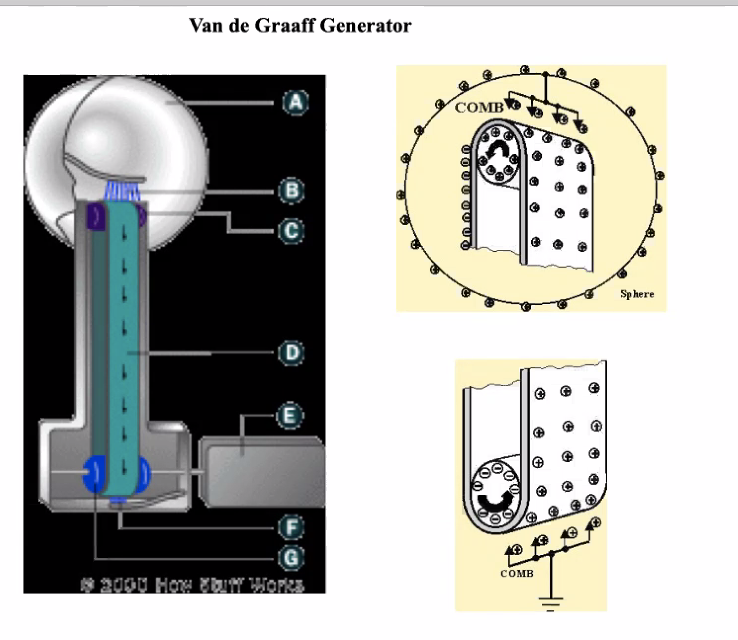
\includegraphics[width=.9\linewidth]{./Screen Shot 2020-09-09 at 10.25.51 AM.png}
\caption{Screen Shot 2020-09-09 at 10.25.51 AM.png}
\end{figure}

\subsection{Basic Procedures}
\label{sec:org27917e2}
\begin{enumerate}
\item User turns crank
\item User brings handle to the globe
\item Electrostatic Bang!
\end{enumerate}

\subsection{But, how does it work?}
\label{sec:org2cd4711}
\begin{itemize}
\item Cranks connects to a white roller, and next to it some metal teeth
\item Roller connnects to transparent belt, and on the other end, under the
globe, there is a similar roller
\item Metal combs next to rollers
\item When cranks are turned, the bottom roller becomes negative, and the
top roller becomes positive
\item So, electron flow between handle (connected to bottom) and globe
(connected to top)
\end{itemize}

\subsection{Why Van de Graff is so exciting}
\label{sec:orga40ac4c}
Van de graff generator so exciting because, unlike normal statics,
charges are added from the inside (see, wire B from the figure)

\begin{itemize}
\item When you add additional changes, because conductor wants to stay 0,
the additional charges can't do anything but accept it
\item Sphere slightly curved to make up for gaping hole
\item Normal door-handle statics would much rater simply eject the added
change as their electric field is pointed at one direction against
charge introduction
\end{itemize}

\subsection{Why are there sparks through the air?}
\label{sec:org6df4b43}
\begin{itemize}
\item One dome that's positive, one dome is negative
\item So, what happens when Spark! happens?

\begin{itemize}
\item Enough charge to overcome the electric field resistance
\href{KBhPHYS201ResistanceConductivity.org}{KBhPHYS201ResistanceConductivity}
of air (like 3.4 million Volts/metre), and \textbf{air ionizes} --- air
atoms becomes so attracted that their electrons ditch their nuclei
and air suddenly becomes a conductors
\item Neutral air has high resistance, but when it ionizes, the air looses
its resistance (drops) and becomes nicely conductive
\item So then, current (Coulomb/s) that flow in the air suddenly spark up
because of sudden loss of resistance, discharging the negative dom
\end{itemize}
\end{itemize}
\end{document}
